\documentclass{article}\usepackage[]{graphicx}\usepackage[]{color}
%% maxwidth is the original width if it is less than linewidth
%% otherwise use linewidth (to make sure the graphics do not exceed the margin)
\makeatletter
\def\maxwidth{ %
  \ifdim\Gin@nat@width>\linewidth
    \linewidth
  \else
    \Gin@nat@width
  \fi
}
\makeatother

\definecolor{fgcolor}{rgb}{0.345, 0.345, 0.345}
\newcommand{\hlnum}[1]{\textcolor[rgb]{0.686,0.059,0.569}{#1}}%
\newcommand{\hlstr}[1]{\textcolor[rgb]{0.192,0.494,0.8}{#1}}%
\newcommand{\hlcom}[1]{\textcolor[rgb]{0.678,0.584,0.686}{\textit{#1}}}%
\newcommand{\hlopt}[1]{\textcolor[rgb]{0,0,0}{#1}}%
\newcommand{\hlstd}[1]{\textcolor[rgb]{0.345,0.345,0.345}{#1}}%
\newcommand{\hlkwa}[1]{\textcolor[rgb]{0.161,0.373,0.58}{\textbf{#1}}}%
\newcommand{\hlkwb}[1]{\textcolor[rgb]{0.69,0.353,0.396}{#1}}%
\newcommand{\hlkwc}[1]{\textcolor[rgb]{0.333,0.667,0.333}{#1}}%
\newcommand{\hlkwd}[1]{\textcolor[rgb]{0.737,0.353,0.396}{\textbf{#1}}}%

\usepackage{framed}
\makeatletter
\newenvironment{kframe}{%
 \def\at@end@of@kframe{}%
 \ifinner\ifhmode%
  \def\at@end@of@kframe{\end{minipage}}%
  \begin{minipage}{\columnwidth}%
 \fi\fi%
 \def\FrameCommand##1{\hskip\@totalleftmargin \hskip-\fboxsep
 \colorbox{shadecolor}{##1}\hskip-\fboxsep
     % There is no \\@totalrightmargin, so:
     \hskip-\linewidth \hskip-\@totalleftmargin \hskip\columnwidth}%
 \MakeFramed {\advance\hsize-\width
   \@totalleftmargin\z@ \linewidth\hsize
   \@setminipage}}%
 {\par\unskip\endMakeFramed%
 \at@end@of@kframe}
\makeatother

\definecolor{shadecolor}{rgb}{.97, .97, .97}
\definecolor{messagecolor}{rgb}{0, 0, 0}
\definecolor{warningcolor}{rgb}{1, 0, 1}
\definecolor{errorcolor}{rgb}{1, 0, 0}
\newenvironment{knitrout}{}{} % an empty environment to be redefined in TeX

\usepackage{alltt}
\usepackage{graphicx}
%% for inline R code: if the inline code is not correctly parsed, you will see a message
\newcommand{\rinline}[1]{SOMETHING WRONG WITH knitr}


\IfFileExists{upquote.sty}{\usepackage{upquote}}{}
\begin{document}

\section{Test}
We have implented testing functions for each method to ensure that each 
function takes proper inputs and returns desired outputs. Each method 
functions properly when tested using small data sets. In order to test the 
functionality of our genetic algorithm, we employed a real-life data set. We 
would like to compare out selected model using genetic algorithim with a 
well-known variable selection mechanism. In our tests, we used stepAIC function. 


The real-life data set was obtained from surveys concerning how video games 
affect grades. There are 15 columns in the data set and grade will be used as  
the dependent variable.


First, we compared our selected model with the model seletced by stepAIC.
The following results are obtained using our genetic algorithim.

\begin{knitrout}
\definecolor{shadecolor}{rgb}{0.969, 0.969, 0.969}\color{fgcolor}\begin{kframe}
\begin{alltt}
\hlstd{data} \hlkwb{<-} \hlkwd{read.table}\hlstd{(}\hlstr{"~/video.txt"}\hlstd{,} \hlkwc{header}\hlstd{=}\hlnum{TRUE}\hlstd{,} \hlkwc{quote}\hlstd{=}\hlstr{"\textbackslash{}""}\hlstd{)}
\hlstd{pop_size} \hlkwb{<-} \hlkwd{min}\hlstd{(}\hlkwd{nrow}\hlstd{(data)}\hlopt{*}\hlnum{2}\hlstd{,} \hlnum{200}\hlstd{)}
\hlstd{ga} \hlkwb{<-} \hlkwd{select_model}\hlstd{(data,}
                   \hlkwc{yvar} \hlstd{=} \hlstr{"grade"}\hlstd{,}
                   \hlkwc{xvars} \hlstd{=} \hlkwd{c}\hlstd{(}\hlstr{"time"}\hlstd{,} \hlstr{"like"}\hlstd{,} \hlstr{"where"}\hlstd{,} \hlstr{"freq"}\hlstd{,} \hlstr{"busy"}\hlstd{,}\hlstr{"educ"}\hlstd{,}
                             \hlstr{"sex"}\hlstd{,} \hlstr{"age"}\hlstd{,} \hlstr{"home"}\hlstd{,} \hlstr{"math"}\hlstd{,} \hlstr{"work"}\hlstd{,} \hlstr{"own"}\hlstd{,}
                             \hlstr{"cdrom"}\hlstd{,} \hlstr{"email"}\hlstd{),}
                   \hlkwc{num_max_iterations} \hlstd{=} \hlnum{35L}\hlstd{,}
                   \hlkwc{model} \hlstd{=} \hlstr{"glm"}\hlstd{,}
                   \hlkwc{seed} \hlstd{=} \hlnum{100}\hlstd{)}
\end{alltt}
\begin{verbatim}
## Initializing population...
## Producing generation 1...
## Producing generation 2...
## Producing generation 3...
## Producing generation 4...
## Producing generation 5...
## Producing generation 6...
## Producing generation 7...
## Producing generation 8...
## Producing generation 9...
## Producing generation 10...
## Producing generation 11...
## Producing generation 12...
## Producing generation 13...
## Producing generation 14...
## Producing generation 15...
## Producing generation 16...
## Producing generation 17...
## Producing generation 18...
## Producing generation 19...
## Producing generation 20...
## Producing generation 21...
## Producing generation 22...
## Producing generation 23...
## Producing generation 24...
## Producing generation 25...
## Producing generation 26...
## Producing generation 27...
## Producing generation 28...
## Producing generation 29...
## Producing generation 30...
## Producing generation 31...
## Producing generation 32...
## Producing generation 33...
## Producing generation 34...
## Producing generation 35...
## Model selection complete!
\end{verbatim}
\begin{alltt}
\hlkwd{summary_ga}\hlstd{(ga,} \hlkwc{num_view} \hlstd{=} \hlnum{3}\hlstd{)}
\end{alltt}
\begin{verbatim}
## Model 1 :
##  grade =  
##  AIC = 157.6 
##  --------------------------------------------------
## Model 2 :
##  grade =  
##  AIC = 158.2 
##  --------------------------------------------------
## Model 3 :
##  grade =  
##  AIC = 158.7 
##  --------------------------------------------------
\end{verbatim}
\end{kframe}
\end{knitrout}


The following results are obtained using stepAIC function.

\begin{knitrout}
\definecolor{shadecolor}{rgb}{0.969, 0.969, 0.969}\color{fgcolor}\begin{kframe}
\begin{alltt}
\hlkwd{library}\hlstd{(MASS)}
\hlstd{mod} \hlkwb{<-} \hlkwd{glm}\hlstd{(grade} \hlopt{~} \hlstd{time} \hlopt{+} \hlstd{like} \hlopt{+} \hlstd{where} \hlopt{+} \hlstd{freq} \hlopt{+} \hlstd{busy} \hlopt{+} \hlstd{educ} \hlopt{+} \hlstd{sex} \hlopt{+} \hlstd{age} \hlopt{+}
            \hlstd{home} \hlopt{+} \hlstd{math} \hlopt{+} \hlstd{work} \hlopt{+} \hlstd{own} \hlopt{+} \hlstd{cdrom} \hlopt{+} \hlstd{email,} \hlkwc{data} \hlstd{= data)}
\hlkwd{stepAIC}\hlstd{(mod)}
\end{alltt}
\begin{verbatim}
## Start:  AIC=167.2
## grade ~ time + like + where + freq + busy + educ + sex + age + 
##     home + math + work + own + cdrom + email
## 
##         Df Deviance AIC
## - age    1     23.6 165
## - where  1     23.6 166
## - time   1     23.6 166
## - like   1     23.7 166
## - educ   1     23.8 166
## - cdrom  1     23.8 166
## - work   1     23.9 166
## - email  1     23.9 167
## - busy   1     23.9 167
## <none>         23.6 167
## - math   1     24.2 168
## - own    1     24.2 168
## - freq   1     24.6 169
## - home   1     25.8 174
## - sex    1     27.4 179
## 
## Step:  AIC=165.3
## grade ~ time + like + where + freq + busy + educ + sex + home + 
##     math + work + own + cdrom + email
## 
##         Df Deviance AIC
## - where  1     23.7 164
## - time   1     23.7 164
## - like   1     23.8 164
## - educ   1     23.8 164
## - cdrom  1     23.8 164
## - work   1     23.9 165
## - busy   1     24.0 165
## - email  1     24.0 165
## <none>         23.6 165
## - math   1     24.2 166
## - own    1     24.3 166
## - freq   1     24.6 167
## - home   1     25.9 172
## - sex    1     27.5 178
## 
## Step:  AIC=163.7
## grade ~ time + like + freq + busy + educ + sex + home + math + 
##     work + own + cdrom + email
## 
##         Df Deviance AIC
## - like   1     23.9 162
## - cdrom  1     23.9 162
## - busy   1     24.0 163
## - time   1     24.0 163
## - work   1     24.0 163
## - educ   1     24.1 164
## - math   1     24.2 164
## <none>         23.7 164
## - email  1     24.2 164
## - own    1     24.4 165
## - freq   1     24.8 166
## - home   1     26.1 170
## - sex    1     27.9 177
## 
## Step:  AIC=162.4
## grade ~ time + freq + busy + educ + sex + home + math + work + 
##     own + cdrom + email
## 
##         Df Deviance AIC
## - cdrom  1     24.1 161
## - time   1     24.2 162
## - work   1     24.2 162
## - busy   1     24.2 162
## - math   1     24.3 162
## - email  1     24.4 162
## - educ   1     24.4 162
## <none>         23.9 162
## - own    1     24.6 163
## - freq   1     25.0 164
## - home   1     26.2 169
## - sex    1     27.9 175
## 
## Step:  AIC=161.2
## grade ~ time + freq + busy + educ + sex + home + math + work + 
##     own + email
## 
##         Df Deviance AIC
## - time   1     24.4 160
## - work   1     24.4 160
## - busy   1     24.5 161
## - math   1     24.5 161
## - educ   1     24.6 161
## <none>         24.1 161
## - email  1     24.6 161
## - own    1     24.7 162
## - freq   1     25.1 163
## - home   1     26.6 168
## - sex    1     28.6 175
## 
## Step:  AIC=160.3
## grade ~ freq + busy + educ + sex + home + math + work + own + 
##     email
## 
##         Df Deviance AIC
## - work   1     24.7 160
## - busy   1     24.8 160
## - email  1     24.8 160
## - educ   1     24.9 160
## - math   1     24.9 160
## <none>         24.4 160
## - own    1     25.0 161
## - freq   1     25.6 163
## - home   1     27.1 168
## - sex    1     28.7 173
## 
## Step:  AIC=159.6
## grade ~ freq + busy + educ + sex + home + math + own + email
## 
##         Df Deviance AIC
## - email  1     25.1 159
## - busy   1     25.2 159
## - own    1     25.2 159
## - educ   1     25.2 159
## <none>         24.7 160
## - math   1     25.8 162
## - freq   1     25.9 162
## - home   1     27.3 167
## - sex    1     28.8 171
## 
## Step:  AIC=159.2
## grade ~ freq + busy + educ + sex + home + math + own
## 
##        Df Deviance AIC
## - own   1     25.5 159
## - educ  1     25.6 159
## - busy  1     25.6 159
## <none>        25.1 159
## - math  1     26.2 161
## - freq  1     26.3 161
## - home  1     27.8 166
## - sex   1     29.2 171
## 
## Step:  AIC=158.6
## grade ~ freq + busy + educ + sex + home + math
## 
##        Df Deviance AIC
## - busy  1     26.0 158
## - educ  1     26.0 158
## <none>        25.5 159
## - math  1     26.6 160
## - freq  1     26.7 161
## - home  1     27.8 164
## - sex   1     29.4 169
## 
## Step:  AIC=158.2
## grade ~ freq + educ + sex + home + math
## 
##        Df Deviance AIC
## <none>        26.0 158
## - freq  1     26.7 159
## - math  1     26.8 159
## - educ  1     27.4 161
## - home  1     28.4 164
## - sex   1     29.8 168
## 
## Call:  glm(formula = grade ~ freq + educ + sex + home + math, data = data)
## 
## Coefficients:
## (Intercept)         freq         educ          sex         home  
##     2.74632      0.00422     -0.00553      0.41845      0.37933  
##        math  
##    -0.00989  
## 
## Degrees of Freedom: 90 Total (i.e. Null);  85 Residual
## Null Deviance:	    33.2 
## Residual Deviance: 26 	AIC: 158
\end{verbatim}
\end{kframe}
\end{knitrout}

The best model found using genetic algorithim included predictors "where",  
"freq","busy", "sex", "home" and "math", yielding AIC of 157.56. This result 
is better than the results we obtained using the stepAIC function. 

Second, we ploted the best AIC for each iteration to see how the AIC score 
has changed over generation. 

\begin{knitrout}
\definecolor{shadecolor}{rgb}{0.969, 0.969, 0.969}\color{fgcolor}\begin{kframe}
\begin{alltt}
\hlkwd{plot.ga}\hlstd{(ga,} \hlkwc{num_view} \hlstd{=} \hlnum{3}\hlstd{)}
\end{alltt}
\end{kframe}
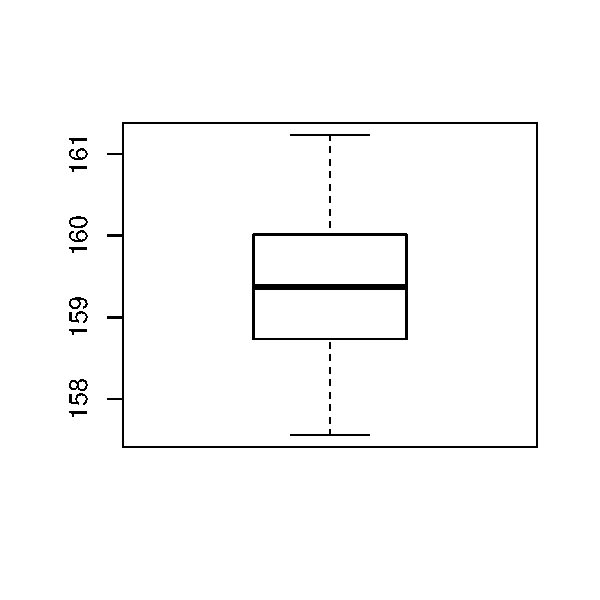
\includegraphics[width=\maxwidth]{figure/latex-unnamed-chunk-31} 

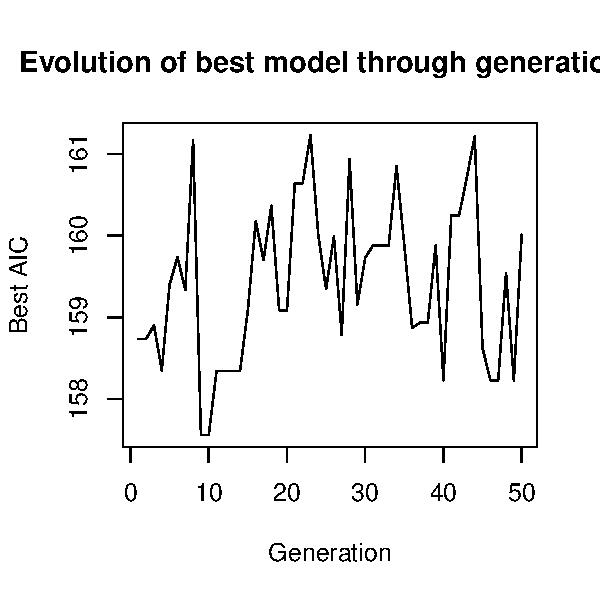
\includegraphics[width=\maxwidth]{figure/latex-unnamed-chunk-32} 

\end{knitrout}

From the box plot, we can see that the AIC ranges from 155 to 165. 
From the Evolution of best model through generations plot, we can see that 
the best model was found around generation 30. 

\end{document}
